\chapter{MNIST}

Die MNIST (Modified National Institute if Standards and Technology) Datenbank ist eine große Datenbank mit handgeschriebenen Ziffer (0..9). Die Datenbank enthält 60.000 Trainingsbilder und 10.000 Testbilder. Als Beispiel siehe Bild \ref{fig:MNIST_multi}
\begin{figure}[!ht]
\centering
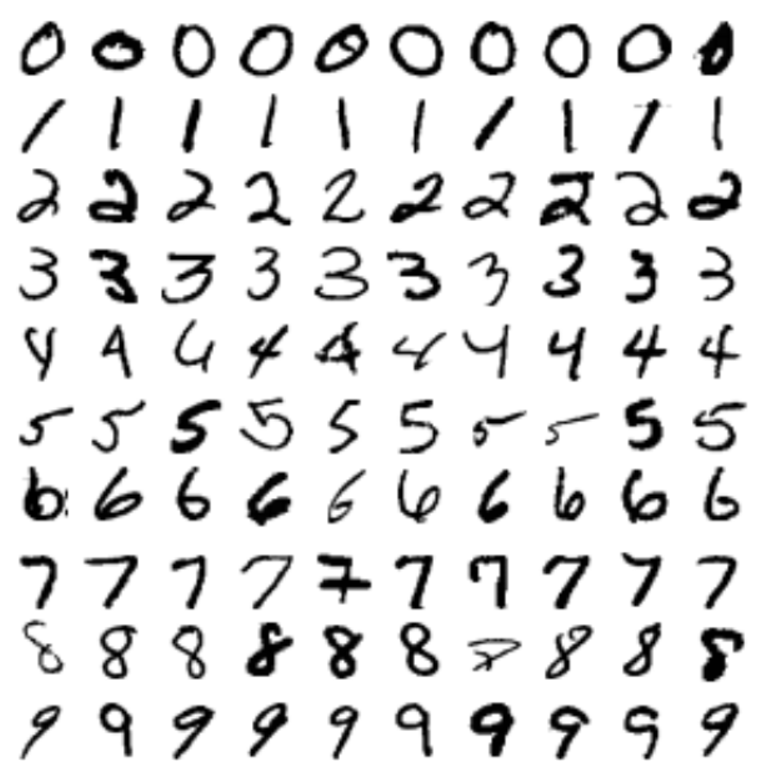
\includegraphics[width=0.5\textwidth]{images/MNIST_multi}
\caption{Ausschnit aus MNIST Datenbank}
\label{fig:MNIST_multi}
\end{figure}

Das Format der Bilder ist dabei 28x28 und besteht aus schwarzer Schrift auf weißem Hintergrund. Ein Pixel kann dabei Werte zwischen 0(weiß) und 1(schwarz) annehmen. ALs Beispiel siehe Bild \ref{fig:MNIST_single}
\begin{figure}[!ht]
\centering
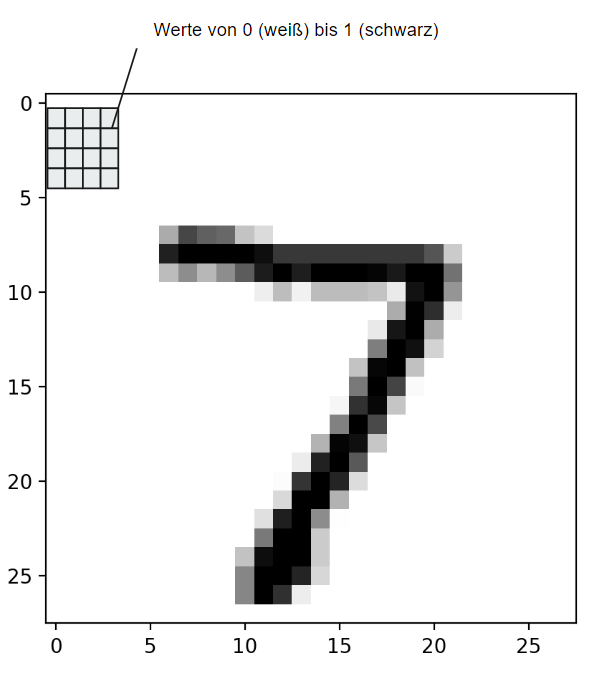
\includegraphics[width=0.5\textwidth]{images/MNIST_single}
\caption{Betrachtung eines einzelnen MNIST Datensets}
\label{fig:MNIST_single}
\end{figure}
Diese Daten werden häufig zum Trainieren und Testen verschiedenster Bilderkennungsmodellen bzw. Algorithmen verwendet. Wir benutzen sie in unserem Beispiel um unserem Modell beizubringen handschriftliche Ziffern zu erkennnen.

\section{Implementierung: MNIST Daten einlesen}
In unserem Codebeispiel ist das einlesen der MNISt Daten auch der erste Schritt der programmiert werden muss. Dazu müssen wir aber generell vorher alle für das Programm benötigten Abhängigkeiten importieren. In unserem Programm werden folgende Abhängigkeiten benötigt:
\lstset{language=Python}
\definecolor{listinggray}{gray}{0.95} 
\definecolor{keyword}{rgb}{0.4, 0, 0.1} 
\definecolor{comment}{rgb}{0, 0.4, 0}
% Zuweisen der Farben zu den entsprechenden Elementen ... 
\lstset{keywordstyle=\color{keyword}\bfseries} 
\lstset{commentstyle=\color{comment}} 
\lstset{backgroundcolor=\color{listinggray}}

\begin{lstlisting}
import tensorflow as tf
import os
import matplotlib as matplotlib
import matplotlib.pyplot as plt
import pandas as pd
from tensorflow.contrib.tensorboard.plugins import projector
\end{lstlisting}
Diese Imports werden ganz oben an den Anfang des Skripts geschrieben.\\
Die MNSIT Daten selbst bekommen wir von Tensorflow, da diese die MNIST Daten in ihre Beispiele integriert haben. Diese Möglickeit des Ladens der Daten könnte in Zukunft ein Problem darstellen, da Tensorflow derzeit ihre Beispielstruktur ändert. Dies Laden der Daten kann mit folgendem Befehl realisiert werden.
\lstset{language=Python}
\definecolor{listinggray}{gray}{0.95} 
\definecolor{keyword}{rgb}{0.4, 0, 0.1} 
\definecolor{comment}{rgb}{0, 0.4, 0}
% Zuweisen der Farben zu den entsprechenden Elementen ... 
\lstset{keywordstyle=\color{keyword}\bfseries} 
\lstset{commentstyle=\color{comment}} 
\lstset{backgroundcolor=\color{listinggray}}

\begin{lstlisting}
from tensorflow.examples.tutorials.mnist import input_data
\end{lstlisting}
Dadurch werden die Trainings und Testdaten automatisch als Archiv heruntergeladen.\\
Es gibt gibt zwei Möglickeiten die Labels der Daten auszulesen. Mann kann sie ganz normal binär interpretieren also zum Beispiel \emph{2=0000000010} oder mit one\char`_hot encoding zum Beispiel \emph{2=0010000000}. Dies lässt sich mit einem mit dem Übergabeparameter der Funktion \emph{input\char`_data.read\char`_data\char`_sets()} einstellen. Setzt man \emph{one\char`_hot=false} wird die normale binäre Version genutzt, setzt man \emph{one\char`_hot=true} verwendet man one\char`_hot encoding. Wir werden unsere Daten mit beiden Möglichkeiten auslesen.
\lstset{language=Python}
\definecolor{listinggray}{gray}{0.95} 
\definecolor{keyword}{rgb}{0.4, 0, 0.1} 
\definecolor{comment}{rgb}{0, 0.4, 0}
% Zuweisen der Farben zu den entsprechenden Elementen ... 
\lstset{keywordstyle=\color{keyword}\bfseries} 
\lstset{commentstyle=\color{comment}} 
\lstset{backgroundcolor=\color{listinggray}}
\begin{lstlisting}
mnist = input_data.read_data_sets("image_data", one_hot=True)
mnistTwo = input_data.read_data_sets("image_data", one_hot=False)
\end{lstlisting}
Um die Daten nachher in Tensorboard verwenden und anzeigen zu können, speichern wir sie noch in eine Variable mit
\lstset{language=Python}
\definecolor{listinggray}{gray}{0.95} 
\definecolor{keyword}{rgb}{0.4, 0, 0.1} 
\definecolor{comment}{rgb}{0, 0.4, 0}
% Zuweisen der Farben zu den entsprechenden Elementen ... 
\lstset{keywordstyle=\color{keyword}\bfseries} 
\lstset{commentstyle=\color{comment}} 
\lstset{backgroundcolor=\color{listinggray}}
\begin{lstlisting}
images = tf.Variable(mnist.test.images, name='images')
\end{lstlisting}
\section{Testen: MNIST Daten einlesen}
Um zu testen ob die Daten richtig heruntergeladen und eingelesen wurden lassen wir uns einfach ein Bild aus den MNIST Daten anzeigen. Der hier folgende Codeblock kann nach dem Testen wieder auskommentiert werden.\\
Dafür lesen wir die Werte eines Bildes aus(hier Bild Nr.240) und reshapen sie von einem 784x1 Vektors zu ener 28x28 Matrix, damit die Pixel wieder an der richtigen Stelle sind.
\lstset{language=Python}
\definecolor{listinggray}{gray}{0.95} 
\definecolor{keyword}{rgb}{0.4, 0, 0.1} 
\definecolor{comment}{rgb}{0, 0.4, 0}
% Zuweisen der Farben zu den entsprechenden Elementen ... 
\lstset{keywordstyle=\color{keyword}\bfseries} 
\lstset{commentstyle=\color{comment}} 
\lstset{backgroundcolor=\color{listinggray}}
\begin{lstlisting}
testImage = mnist.test.images[240].reshape(28,28)
\end{lstlisting}
Diese Matrix lassen wir dann mit dem Package Matplotlib auf einen Plot printen mit folgendem Befehl:
\begin{lstlisting}
plt.imshow(testImage, cmap = matplotlib.cm.binary, interpolation = "nearest")
\end{lstlisting}
Um zu wissen welche Ziffer ausgegeben wird lassen wir auch noch das Label ausgeben
\begin{lstlisting}
print(mnist.test.labels[240])
\end{lstlisting}
Und dann müssen wir noch den Plot ausgeben
\begin{lstlisting}
plt.show()
\end{lstlisting}
Funktioniert dies, sollte diese Codestück wieder auskommentiert oder gelöscht werden.

\label{cha:MNIST}